\documentclass[tikz,border=8pt]{standalone}
\usepackage{fontspec}
\usepackage{xcolor}
\usetikzlibrary{arrows.meta,positioning,shapes.geometric,calc}

\definecolor{htnblue}{RGB}{52,101,164}
\definecolor{morlred}{RGB}{180,70,60}
\definecolor{gamegreen}{RGB}{72,128,92}
\definecolor{fallbackorange}{RGB}{196,120,45}
\definecolor{envgray}{RGB}{100,100,100}

\begin{document}
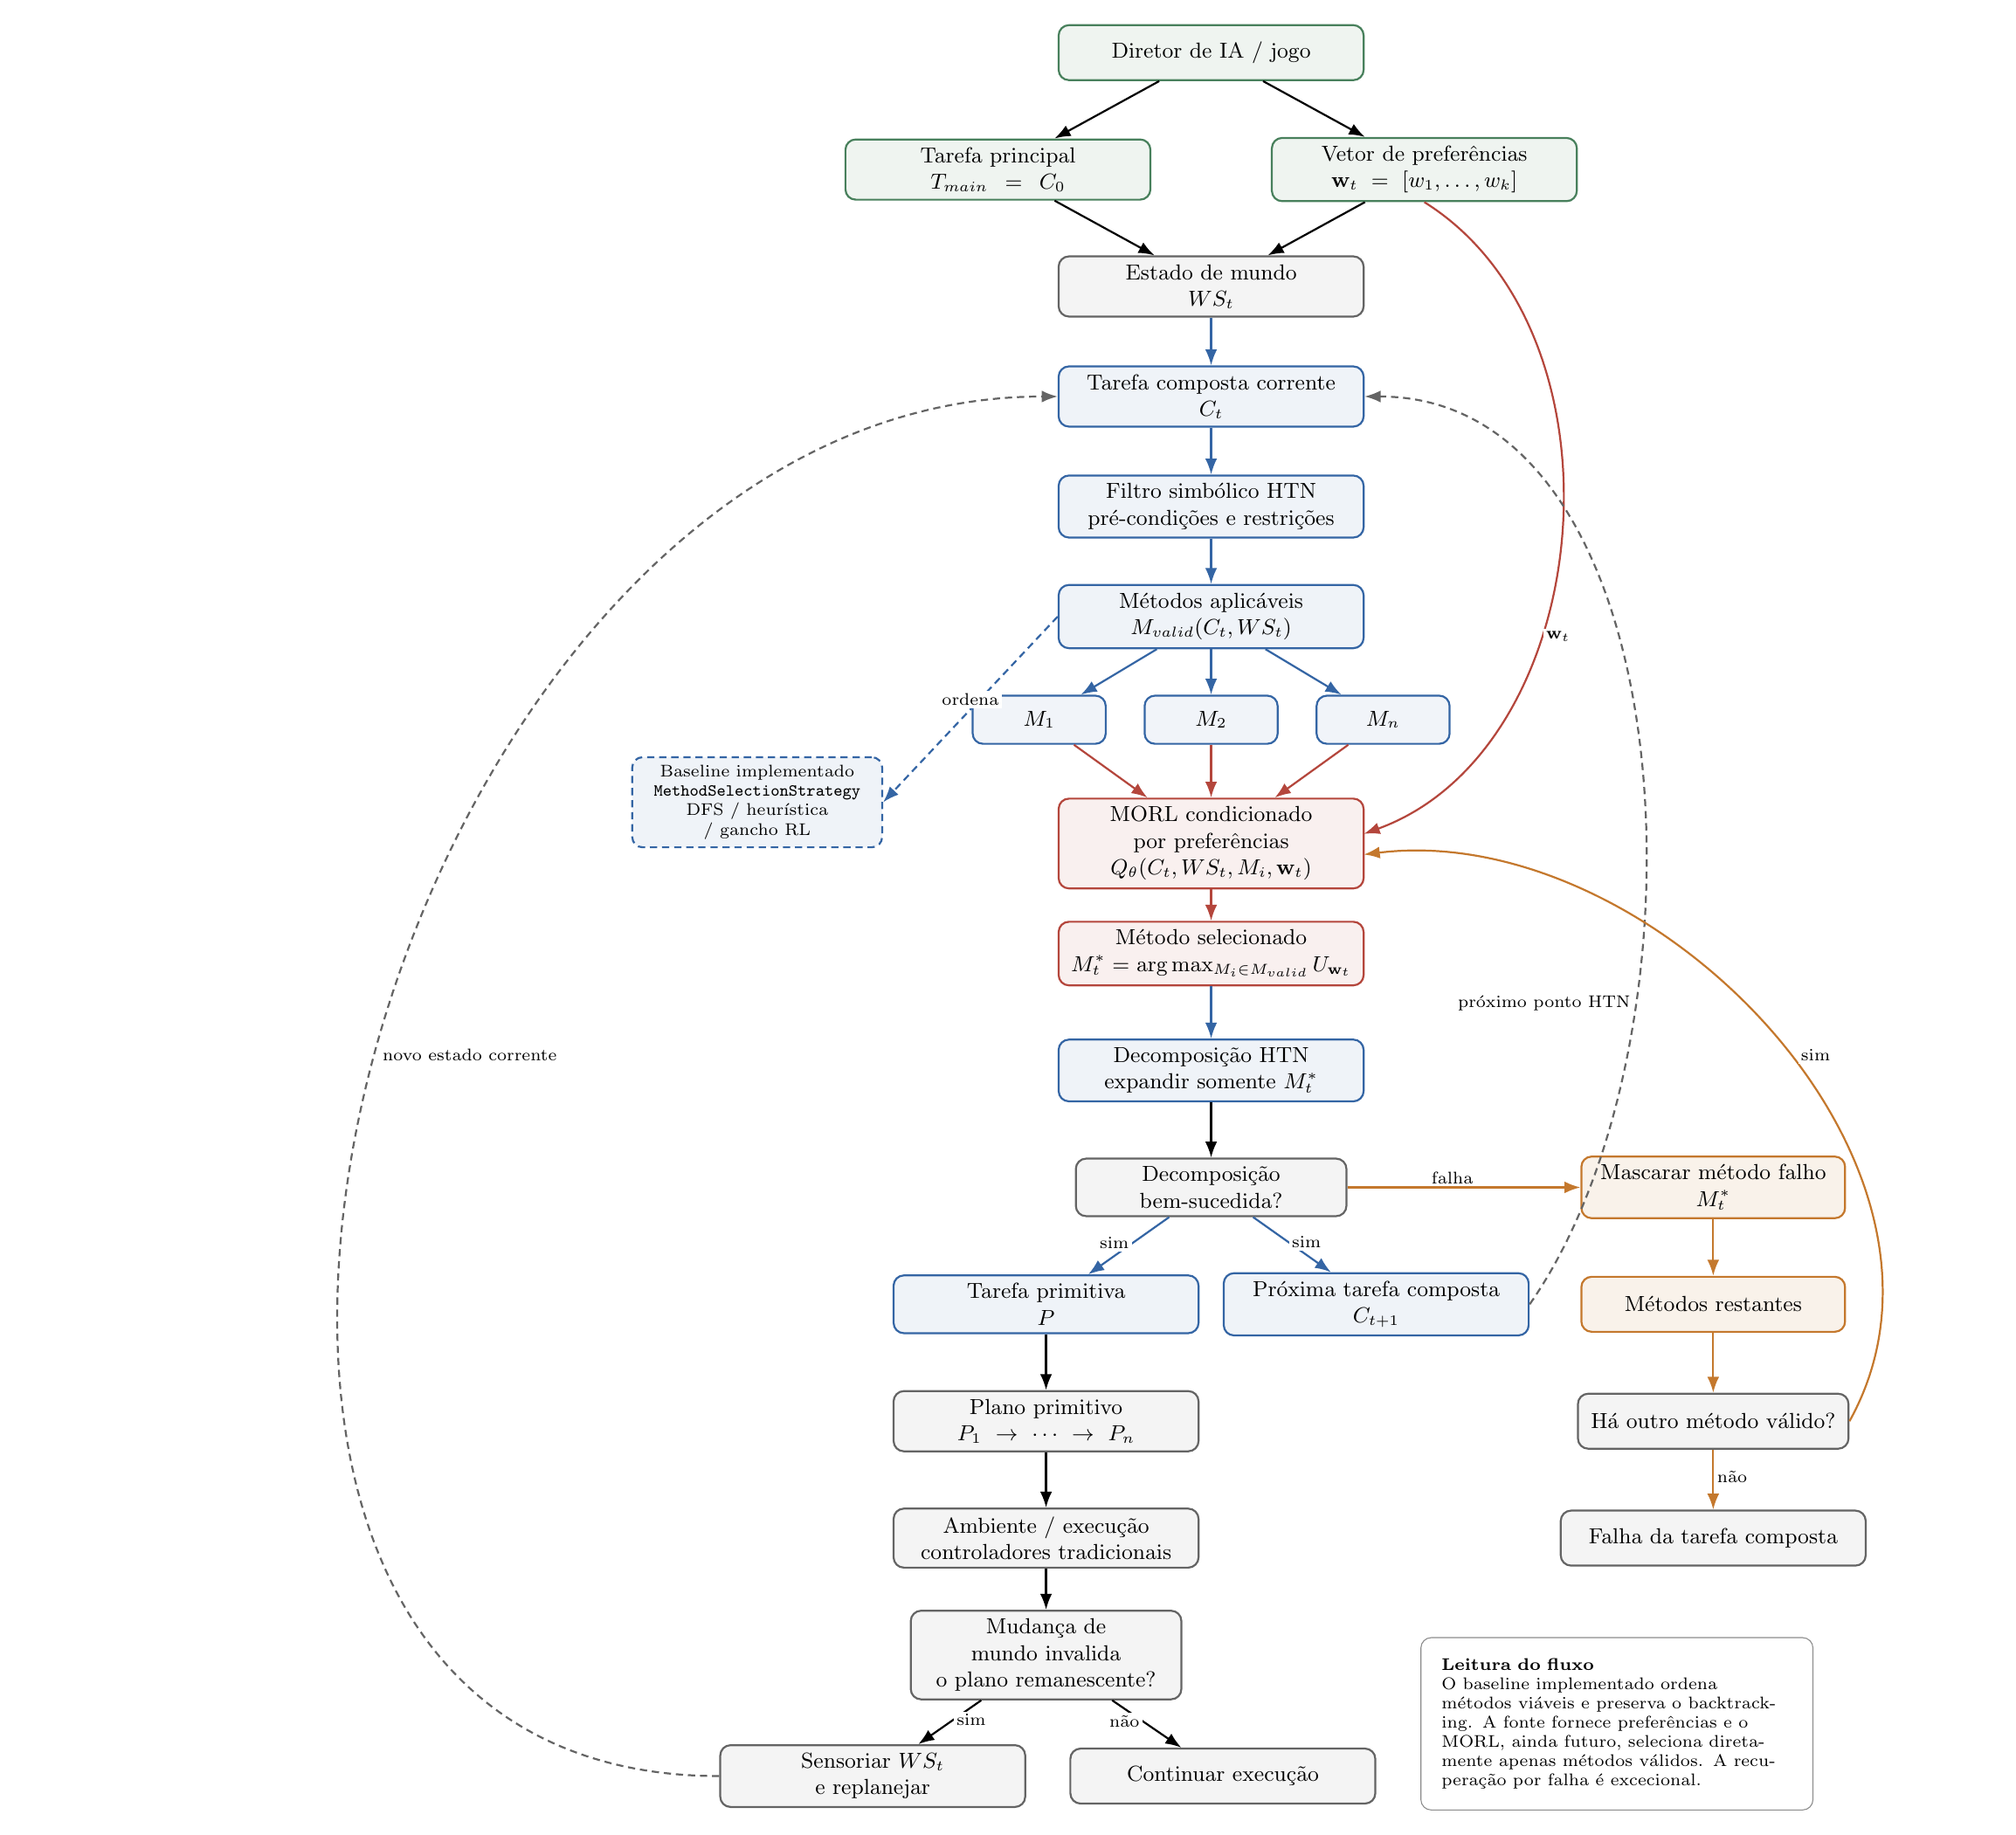
\begin{tikzpicture}[
  font=\small,
  >=Latex,
  node distance=7mm,
  block/.style={rectangle, rounded corners=1.5mm, draw, thick, align=center,
    text width=42mm, minimum height=8mm},
  game/.style={block, draw=gamegreen, fill=gamegreen!9},
  htn/.style={block, draw=htnblue, fill=htnblue!8},
  morl/.style={block, draw=morlred, fill=morlred!8},
  runtime/.style={block, draw=envgray, fill=envgray!7},
  fallback/.style={block, draw=fallbackorange, fill=fallbackorange!10},
  smallblock/.style={rectangle, rounded corners=1.5mm, draw=htnblue, thick,
    fill=htnblue!7, align=center, text width=17mm, minimum height=7mm},
  decision/.style={rectangle, rounded corners=1.5mm, draw=envgray, thick,
    fill=envgray!7, align=center, text width=37mm, minimum height=8mm},
  labeltext/.style={font=\scriptsize, fill=white, inner sep=1.2pt, align=center},
  arrow/.style={->, thick},
  htnarrow/.style={->, thick, draw=htnblue},
  morlarrow/.style={->, thick, draw=morlred},
  fallbackarrow/.style={->, thick, draw=fallbackorange},
  feedback/.style={->, thick, densely dashed, draw=envgray}
]
  % Intenção e estado.
  \node[game] (director) at (0,0) {Diretor de IA / jogo};
  \node[game] (mission) at (-3.1,-1.7) {Tarefa principal\\$T_{main}=C_0$};
  \node[game] (weights) at (3.1,-1.7) {Vetor de preferências\\$\mathbf{w}_t=[w_1,\ldots,w_k]$};
  \node[runtime] (state) at (0,-3.4) {Estado de mundo\\$WS_t$};
  \node[htn] (compound) at (0,-5.0) {Tarefa composta corrente\\$C_t$};
  \node[htn] (filter) at (0,-6.6) {Filtro simbólico HTN\\pré-condições e restrições};
  \node[htn] (valid) at (0,-8.2) {Métodos aplicáveis\\$M_{valid}(C_t,WS_t)$};
  \node[smallblock] (mone) at (-2.5,-9.7) {$M_1$};
  \node[smallblock] (mtwo) at (0,-9.7) {$M_2$};
  \node[smallblock] (mn) at (2.5,-9.7) {$M_n$};
  \node[htn, densely dashed, text width=34mm, font=\scriptsize] (baseline) at (-6.6,-10.9)
    {Baseline implementado\\\texttt{MethodSelectionStrategy}\\DFS / heurística / gancho RL};
  \node[morl] (selector) at (0,-11.5) {MORL condicionado por preferências\\$Q_\theta(C_t,WS_t,M_i,\mathbf{w}_t)$};
  \node[morl] (selected) at (0,-13.1) {Método selecionado\\$M_t^*=\arg\max_{M_i\in M_{valid}} U_{\mathbf{w}_t}$};
  \node[htn] (decompose) at (0,-14.8) {Decomposição HTN\\expandir somente $M_t^*$};
  \node[decision] (success) at (0,-16.5) {Decomposição bem-sucedida?};

  % Caminho normal de execução.
  \node[htn] (primitive) at (-2.4,-18.2) {Tarefa primitiva\\$P$};
  \node[htn] (next) at (2.4,-18.2) {Próxima tarefa composta\\$C_{t+1}$};
  \node[runtime] (plan) at (-2.4,-19.9) {Plano primitivo\\$P_1\rightarrow\cdots\rightarrow P_n$};
  \node[runtime] (execute) at (-2.4,-21.6) {Ambiente / execução\\controladores tradicionais};
  \node[decision] (changed) at (-2.4,-23.3) {Mudança de mundo invalida\\o plano remanescente?};
  \node[runtime] (continue) at (0.17,-25.06) {Continuar execução};
  \node[runtime] (replan) at (-4.92,-25.06) {Sensoriar $WS_t$\\e replanejar};

  % Recuperação excepcional de falha.
  \node[fallback, text width=36mm] (mask) at (7.3,-16.5) {Mascarar método falho\\$M_t^*$};
  \node[fallback, text width=36mm] (remaining) at (7.3,-18.2) {Métodos restantes};
  \node[decision] (any) at (7.3,-19.9) {Há outro método válido?};
  \node[runtime] (failure) at (7.3,-21.6) {Falha da tarefa composta};

  % Fluxo de intenção e observação.
  \draw[arrow] (director) -- (mission);
  \draw[arrow] (director) -- (weights);
  \draw[arrow] (mission) -- (state);
  \draw[arrow] (weights) -- (state);
  \draw[htnarrow] (state) -- (compound);
  \draw[htnarrow] (compound) -- (filter);
  \draw[htnarrow] (filter) -- (valid);
  \draw[htnarrow] (valid) -- (mone);
  \draw[htnarrow] (valid) -- (mtwo);
  \draw[htnarrow] (valid) -- (mn);
  \draw[htnarrow, densely dashed] (valid.west) --
    node[labeltext, pos=.5, above] {ordena} (baseline.east);
  \draw[morlarrow] (mone) -- (selector);
  \draw[morlarrow] (mtwo) -- (selector);
  \draw[morlarrow] (mn) -- (selector);
  \draw[morlarrow] (weights.south) to[out=328, in=20] node[labeltext, pos=.62, below right] {$\mathbf{w}_t$} (2.22,-11.36);
  \draw[morlarrow] (selector) -- (selected);
  \draw[htnarrow] (selected) -- (decompose);
  \draw[arrow] (decompose) -- (success);

  % Saídas e replanejamento.
  \draw[htnarrow] (success) -- node[labeltext, pos=.45, left] {sim} (primitive);
  \draw[htnarrow] (success) -- node[labeltext, pos=.45, right] {sim} (next);
  \draw[arrow] (primitive) -- (plan);
  \draw[arrow] (plan) -- (execute);
  \draw[arrow] (execute) -- (changed);
  \draw[arrow] (changed) -- node[labeltext, pos=.45, left] {não} (continue);
  \draw[arrow] (changed) -- node[labeltext, pos=.45, right] {sim} (replan);
  \draw[feedback] (replan.west) to[out=180, in=180, looseness=1.25]
    node[labeltext, pos=.52, below right] {novo estado corrente} (compound.west);
  \draw[feedback] (next.east) to[out=55,in=0,looseness=.9]
    node[labeltext, pos=.28, above left] {próximo ponto HTN} (compound.east);

  % Recuperação de falha, fora do caminho normal.
  \draw[fallbackarrow] (success) -- node[labeltext, pos=.45, above] {falha} (mask);
  \draw[fallbackarrow] (mask) -- (remaining);
  \draw[fallbackarrow] (remaining) -- (any);
  \draw[fallbackarrow] (any) -- node[labeltext, pos=.45, right] {não} (failure);
  \draw[fallbackarrow] (any.east) to[out=61, in=7] node[labeltext, pos=.45, above right ] {sim} (2.22,-11.66);

  \node[draw=black!45, rounded corners=1.5mm, align=left, font=\scriptsize,
    text width=51mm, inner sep=3mm] at (5.9,-24.3) {\textbf{Leitura do fluxo}\\
    O baseline implementado ordena métodos viáveis e preserva o backtracking.
    A fonte fornece preferências e o MORL, ainda futuro, seleciona diretamente
    apenas métodos válidos.
    A recuperação por falha é excecional.};
\end{tikzpicture}
\end{document}
